日本において地上気象観測は古くから行われている。近年では自動気象データ収集システム
(AMeDAS)や、C バンドレーダー・X バンドレーダーの全国配備が進んでいる。
これにより気温・気圧などの気象パラメータと降水分布がほぼリアルタイムに観測される
ような態勢が確立されている。しかしながらこのような最先端の気象観測網をもってしても、
ゲリラ豪雨や線状降水帯、さらには台風に伴う豪雨などといった極端気象現象の予測は
依然として難しい。
気象庁のホームページ\url{https://www.jma.go.jp/jma/kishou/know/yougo_hp/kousui.html}
では降雨の内、「著しい災害が発生した顕著な大雨現象」と豪雨としている。一方、集中豪
雨を「同じような場所で数時間にわたり強く降り、100mm から数百 mm の雨量をもたらす
雨」と説明している。これらのような極端降雨現象は、最先端の技術でも予測が大変難しい
ことで知られている。集中豪雨の中でも、稀にしか発生しないような大雨は極端豪雨・極
端降雨気象などと呼ばれる。
近年における状況をMasaki[2020]の発表をもとにまとめる。気象庁における統計
データ[1]では、1時間降水量が50、80、200、400mm以上の降雨の年間発生件数の、
1975 年以降の変化傾向はいずれにおいても増加トレンドにあることが示されて
いる。(図1)

\begin{figure}[H]
	\begin{tabular}{cc}
		\begin{minipage}[t]{1.0\hsize}
		\begin{center}
		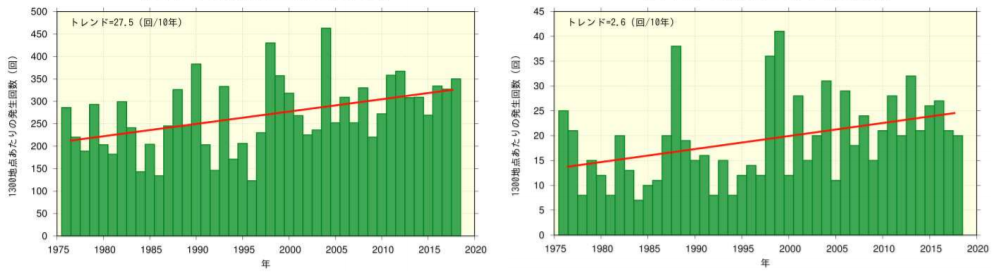
\includegraphics[width=1.0\linewidth,clip]{fig/intro/kisyotyo-repo-chart50-80.png}
		\subcaption{50mm(左)、80mm(右)}
		\label{a}
		\end{center}
		\end{minipage}\\
		
		\begin{minipage}[t]{1.0\hsize}	
		\begin{center}
		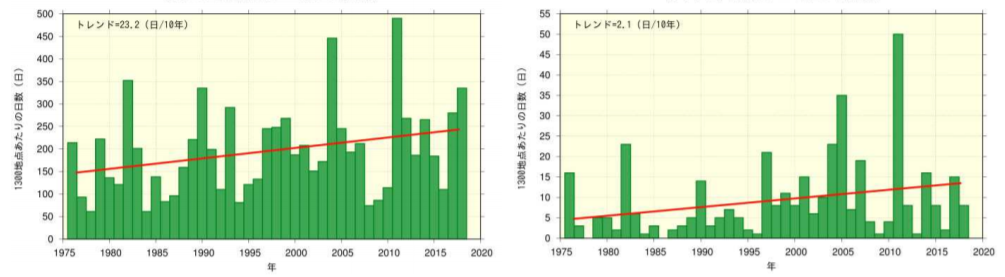
\includegraphics[width=1.0\linewidth,clip]{fig/intro/kisyotyo-repo-chart200-400.png}
		\subcaption{200mm(左)、400mm(右)}
		\label{b}
		\end{center}
		\end{minipage}
	\end{tabular}
	\caption{1976-2018年期間の全国のアメダスの1時間降水量50mm、80mm (a)、200mm、400mm (b) 以上の年間発生回数の変化。棒グラフは全国のアメダスによる観測値を 1300 地点当たりに換算した値、直線は長期変化傾向を表す。}
\end{figure}

Fumikai \textit{et al}.[2006]は、国内51地点の104年間(1901~2004年)の日降水量の資料
から日降水量の降水階級、100mm以上の日数、年最大降水量、年間の上位100事例の
発生頻度等の様々な大雨の尺度を用いて経年変化を調べた。いずれの尺度においても大雨の数は
増加傾向にあることがわかる。

\begin{figure}[H]
\begin{center}
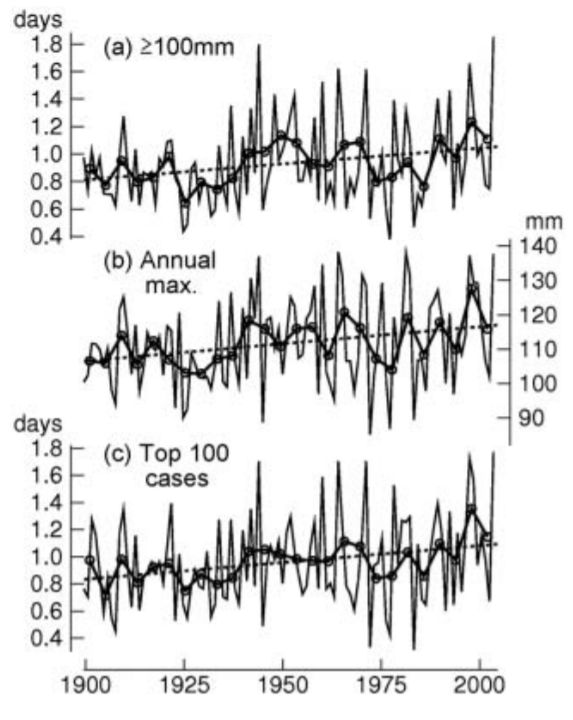
\includegraphics[width=0.8\linewidth]{fig/intro/fumikai-et-al-chart1.png}
\caption{1901-2004年期間の極端豪雨の経年変化:100mm以上の日数、年最大降水量、累年の上位100事例の発生頻度の時系列を示す。横軸は年。}
\end{center}
\end{figure}

日本における極端豪雨の事例のうち、甚大な被害を起こした現象については気象庁が名称を定めている。(表1)

\begin{table}[H]
\renewcommand{\arraystretch}{1.5}
\small
\caption{平成以降に気象庁が定めた気象現象からの豪雨事例(気象庁ホームページ: \protect\url{https://www.jma.go.jp/jma/kishou/know/meishou/meishou_ichiran.html}より改変)}
\label{table:JapanExtremeRainfalls}
\centering
\begin{tabularx}{\textwidth}{>{\hsize=.5\hsize}X>{\hsize=.5\hsize}XX}
\hline
名称 & 期間・現象等 & 「地域独自の名称等」、主な被害 \\
\hline \hline
平成16年7月新潟・福島豪雨 & 平成16年7月17日~13日 & 「7.13 新潟豪雨」。 \\
平成16年7月福井豪雨 & 平成16年7月17日~18日 & 福井県の浸水害・土砂災害等。 \\
平成18年7月豪雨 & 平成18年7月15日~24日 & 「平成18年7月鹿児島県北部豪雨」。諏訪湖(長野県)周辺の土砂災害、浸水害、天竜川(長野県)の氾濫等。 \\
平成20年8月末豪雨 & 平成20年8月26日~31日 & 名古屋市・岡崎市(愛知県)の浸水被害等。 \\
平成21年7月中国・九州北部豪雨 & 平成21年7月19日~26日 & 「平成21年7月21日豪雨」、「山口豪雨災害」 \\
平成23年7月新潟・福島豪雨 & 平成23年7月27日~30日 & 五十嵐川・阿賀野川(新潟県)の氾濫等。 \\
平成24年7月九州北部豪雨 & 平成24年7月11日~14日 & 「熊本広域大水害」、「7.12 竹田市豪雨災害」。八女市(福岡県)、竹田市(大分県)の土砂災害・洪水被害、矢部川(福岡県)の氾濫等。 \\
平成26年8月豪雨 & 平成26年7月30日~8月26日 & 「広島豪雨災害」、「8.20 土砂災害」、「2014 年 8 月広島大規模土砂災害」、「丹羽市豪雨災害」、「2014高知豪雨」。 \\
平成27年9月関東・東北豪雨 & 平成27年9月9日~11日 & 「鬼怒川水害」。鬼怒川(茨城県)・渋井川(宮城県)の氾濫等。 \\
平成29年7月九州北部豪雨 & 平成29年7月5日~6日 & 朝倉市・東峰村(福岡県)・日田市(大分県)の洪水・土砂災害等。 \\
平成30年7月豪雨 & 平成30年6月28日~7月8日 & 「西日本豪雨」。広島県・愛媛県の土砂災害、倉敷市真備町(岡山県)の洪水害など、広域的な被害。 \\
令和元年房総半島台風 & 令和元年9月(台風15号) & 房総半島を中心とした各地で暴風等による被害。台風「ファクサイ」。 \\
令和元年東日本台風 & 令和元年10月(台風19号) & 東日本の広い範囲における記録的な大雨により大河川を含む多数の河川氾濫等による被害。台風「ハギビス」 \\
令和2年7月豪雨 & 令和2年7月3日~31日 & 「熊本豪雨」。西日本から東日本の広範囲にわたる長期間の大雨。球磨川(熊本県)などの河川氾濫や土砂災害による被害。 \\
\hline
\end{tabularx}
\end{table}

平成16年以降、ほぼ毎年のように極端豪雨が発生しており近年極端豪雨が増加していることがわかる。
特に、令和2年7月豪雨では大規模な線状降水帯が発生し甚大な被害を与えたことは記憶に新しい。
近年この「線状降水帯」が原因の極端豪雨の発生が増加しており、そのメカニズムや予測研究が盛んに行われている。
このような極端豪雨が増加している原因の1つとして、地球温暖化があげられている。
気象庁が毎年発表している業務評価レポート[2]では、該当年の降水短時間予報の精度が公表されている。2019年度の予測精度は 0.52 であった。
降水短時間予報は、1 時間10mm以上を超えるやや強い降水に対する降水量の予測である。
降水短時間予報が2時間後から3時間後までの1時間に降ると予測した1km格子ごとの降水量を、
5km格子ごとの値に平均した値を予測値として、同様に1km格子ごとの解析雨量を5km格子ごとの
値に平均した値を実況値とした。これらの予測値と実況値の合計が20mm以上の場合に、予測値と
実況値のうち大きな方を分母として比を計算、5km格子ごとに計算した比を日本の陸上付近で1年
にわたって平均した値が精度となる。このことからも、今もなお、最新の観測・予測技術を
もってしても、極端豪雨を含めた強い雨を正確に予測することは難しいことが示されている。

極端豪雨の予測が難しい主な原因として、Sato[2020]の中では以下のように説明されてい
る。

\begin{quote}
“(前略)長時間の時間スケールにおいては、エネルギー収支によって降水量は制約され
ており、水蒸気が大気中で凝結する際に放出する潜熱と大気中の放射冷却のバランスによ
って説明される。(中略)しかしこのようなバランスは、長時間の広領域で平均した関係で
あるため、個々の降水イベント、とくに極端豪雨に関してはこのようなバランスは成り立た
ない。
(中略)集中豪雨は、一般に数十 km スケールのメソ対流システム(Meso-scale Convective
System : MCS)によってもたらされる。これらは台風や温帯低気圧、梅雨の前線といった
千 km スケールの相関規模の擾乱の内部で発生し、さらに、より大きな 1 万 km スケールの
大気循環(モンスーン循環やハドレー循環等)の大規模場の変化がこれらの総観規模の擾乱
の変調をもたらす。
” [Sato, 2020, p.144]
\end{quote}

すなわち、極端豪雨はその空間的かつ時間的なスケールが小さいために予測を難しくし
ているといわれている。気象観測の先進国である日本であっても予測は困
難であり、気象観測インフラがより脆弱な東南アジア域では、極端気象・極端豪雨の予測は
さらに困難な問題となる。加えて毎年のように甚大な災害を引き起こしており、これから
も社会インフラや人間活動を守る対策として、さらに SDGs(Sustainable Development
Goals)の観点からも、極端気象の予測は急務の課題となっている。
